\pagenumbering{gobble}
\documentclass[letterpaper,12pt]{article}
%% Language and font encodings
\usepackage[english]{babel}
%\usepackage[utf8x]{inputenc}
\usepackage[T1]{fontenc}
\usepackage[compact]{titlesec}
\usepackage{enumitem}
\usepackage{graphicx}
\usepackage{array}
\usepackage{ragged2e}
\usepackage{caption}
\usepackage{subcaption}
\newcolumntype{P}[1]{>{\RaggedRight\hspace{0pt}}p{#1}}
\usepackage[font={footnotesize}]{caption}
\captionsetup[sub]{font=footnotesize,justification=raggedright}

\titlespacing{\section}{0pt}{0pt}{-4pt}
\titlespacing{\subsection}{0pt}{0pt}{-4pt}
\titlespacing{\subsubsection}{0pt}{0pt}{-4pt}

\titleformat{\section}{\normalfont\fontsize{14}{15}\bfseries}{\thesection}{1em}{}
\titleformat{\subsection}{\normalfont\fontsize{12}{15}\bfseries}{\thesubsection}{1em}{}
\titleformat{\subsubsection}{\normalfont\fontsize{12}{15}\bfseries}{\thesubsubsection}{1em}{}


%% Sets page size and margins
\usepackage[letterpaper,top=2.5cm,bottom=2.5cm,left=2.5cm,right=2.5cm,marginparwidth=1.75cm]{geometry}

\renewcommand{\floatpagefraction}{.8}%
%\captionsetup[subfigure]{labelformat=empty}

%% Useful packages
\usepackage{amsmath}
\usepackage{amsmath,tabularx}

\usepackage{graphicx}
\usepackage[colorinlistoftodos]{todonotes}
%\usepackage{color}{hyperref}
%\usepackage[style=authoryear,sorting=ynt,autocite=inline]{biblatex}
%\usepackage[sorting=none]{biblatex}

\usepackage{csquotes}


\title{An overview of key fundamental physical processes which influence atmospheric rivers}
\author{Elizabeth E. McClenny \protect\\ Atmospheric Science Graduate Group \protect\\ University of California, Davis \protect\\ \protect\\ \ PhD Qualifying Exam Committee: \protect\\ \protect\\ \ Dr. Shuhua Chen \protect\\  Dr. Richard Grotjahn  \protect\\ \ Dr. Travis O'Brien \protect\\ Dr. Ashley Payne \protect\\ Dr. Paul Ullrich}

\date{September 30, 2018}

\setlength{\parskip}{1em}

\begin{document}
\raggedright
\maketitle
\pagenumbering{gobble}
\newpage
\tableofcontents
\pagenumbering{gobble}
\newpage
\pagenumbering{arabic}


\section{Introduction}

Transient, filamentary corridors of enhanced vapor transport called atmospheric rivers (ARs) provide virtually all ($\geq$ 90\%) of the poleward vapor transport in the extratropics despite only covering about 10\% of the Earth's zonal circumference \cite{Zhu1998}. ARs provide an estimated 22\% of the Earth's annual global water runoff, bringing water resources to 300 million people \cite{Paltan2017}. For many communities, a wet season with fewer-than-average ARs means drought, while a season with a higher count or stronger ARs than average can mean devastating floods \cite{Dettinger2011}. In all, ARs have consequences from the global hydrologic cycle to local water resources, making them a topic ripe for dissection and discussion.

In order to describe the processes surrounding ARs, we first describe their ``anatomy''. Figures \ref{AR1a} and \ref{AR1b} present schematic views of ARs \footnote{These figures are clipped from the American Meteorology Society (AMS) AR definition page: http://glossary.ametsoc.org/wiki/Atmospheric_river}. These schematics are derived from dropsonde observations deployed from research aircraft, as well as reanalysis output. While the observations and reanalyses come from multiple events, we emphasize here that they may not represent all AR events. However, for the purposes of this paper, we focus on it as our representative AR. Figure \ref{AR1a} shows the AR as a plume of enhanced integrated vapor transport (IVT; color scale) on the leading edge of the cold front of an extratropical cyclone (ETC). Figure \ref{AR1b} presents a cross-section of a representative AR, as well as its associated cold front and low-level jet. 

\begin{figure}[h]
\centering
\begin{subfigure}{.5\textwidth}
  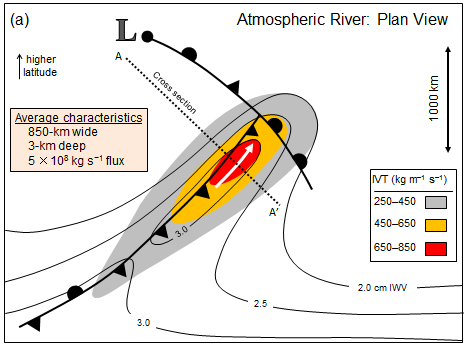
\includegraphics[width=0.8\linewidth]{Atmospheric_river_fig1a.png}
  \caption{Figure 1a: Plan view perspective of AR and parent extratropical cyclone. Color scale is IVT (kgm$^{-1}$s$^{-1}$); contours are vertically-integrated \\ water vapor (IWV; cm).}\label{AR1a}

\end{subfigure}%
\begin{subfigure}{0.5\textwidth}
  \centering
  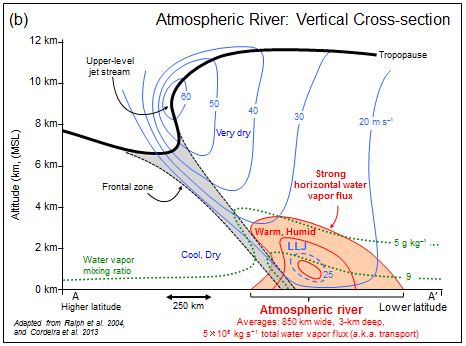
\includegraphics[width=0.8\linewidth]{Atmospheric_river_fig1b.png}
    \caption{Figure 1b: Vertical cross-section of AR. Orange color fill is IVT core; blue isotachs (ms$^{-1}$) are normal to cross-section; green dotted contours are water vapor mixing ratio (gkg$^{-1}$).\\}\label{AR1b}
\end{subfigure}
\end{figure}

\noindent
\begin{tabularx}{\linewidth}{XXX}

\begin{equation} \label{1}
   	IVT =  - \frac{1}{g} \int^{200}_{1000} q \cdot \overrightarrow{u} dp 
\end{equation}
& 
\begin{equation} \label{2}
	IWV = - \frac{1}{\rho g} \int^{200}_{1000} q dp 
\end{equation}

\end{tabularx}

{\footnotesize Calculation for IVT (1) and IWV (2) where $\rho$ is the density of water, $g$ is the gravitational constant, $q$ is water vapor mixing ratio, and $\protect\overrightarrow{u}$ is horizontal wind velocity.}


The rest of this document proceeds as follows: first, synoptic-scale dynamics are described; we move on from here to thermodynamic mechanisms and constraints for ARs; this is followed with a discussion of relevant boundary layer processes; finally, we conclude with a section on potential climate change influences on ARs. %Each of the following sections will begin with a brief description of the fundamental concepts, but will move on from there to describe the relevance of these concepts to ARs. Note that this document does not provide a review of the literature on ARs, but synthesizes fundamental physical concepts and uses ARs as a tool to contextualize them.  

% \begin{figure}[h]
% \centering
%  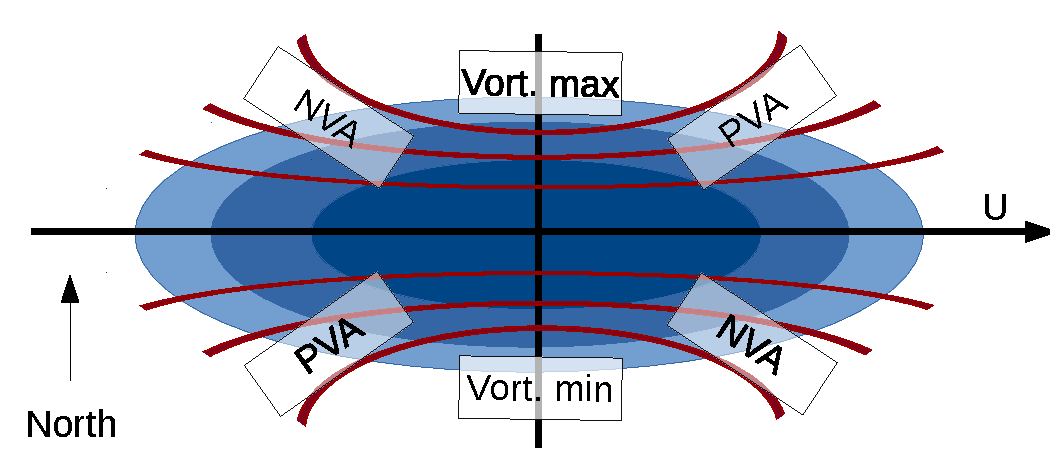
\includegraphics[width=0.6\linewidth]{jetstreak.pdf}
%  \caption{Four-quadrant model for a straight jet streak. The arrow shows the jet streak direction while filled contours are isotachs. Thick red lines are geopotential height contours. Section 2.4 contains a short discussion of the quasigeostrophic forcing by a straight jet streak.}\label{streak}
%  \end{figure}

% \subsection{Midlatitude surface weather}

% %\textbf{Tropical cyclones} (TCs): Rapidly rotating closed low pressure systems which form over warm ocean waters and are fueled by LH release. Especially severe ones can become hurricanes. TCs may undergo \textit{extratropical transition} as they move into the midlatitudes, turning in to extratropical cyclones. 

% \textbf{Extratropical cyclones} (ETCs): Low pressure systems on the surface which drive much of the weather in the midlatitudes. They may originate as tropical cyclones which underwent extratropical transition, or by the process of \textit{midlatitude cyclogenesis}, described below. ETCs are associated with frontal weather systems.

% \textbf{Surface fronts:} Long ($\mathcal{O}(1000 \textrm{km})$), narrow ($\mathcal{O}(100 \textrm{km})$) regions across which the temperature dramatically changes. Note that these dimensions place surface fronts into both the synoptic and mesoscale meteorological regimes, depending on if one is concerned with the along- or across-front characteristics, respectively.

% \textbf{Warm front:} A frontal region across which temperature increases. They tend to exist on the eastern edge of ETCs and move poleward, bringing warm equatorial air with them. The relatively low density of the warm air typically causes warm fronts to move more slowly than cold fronts. Precipitation associated with warm fronts tends to be gentler than that associated with cold fronts. The ETC's \textit{warm sector}, a region of relatively warm, moist air, exists behind the warm front. The warm sector rises above the warm front in a \textit{warm conveyor belt} (WCB). 

% \textbf{Cold front:} A frontal region across which temperature decreases. Cold fronts often exist on the equatorward edge of ETCs and move east, bringing cold polar air to lower latitudes. The density of the cold air allows it to displace air in the warm sector rapidly as it moves, allowing it to ``catch up'' to the warm front in a process known as occlusion. 

% %\textbf{Occluded front:} A frontal region across which a relatively weak temperature change takes place. Often said to occur under the process of occlusion, whereby the cold front ``catches up'' to the slower warm front. 

% \subsection{Quasigeostrophic forcing by jet streaks}\label{MC}

% %\textbf{At the surface:} By \textit{polar front theory}, midlatitude cyclones form along the stationary polar front, at the boundary of the Ferrell and polar cells. An upper-level disturbance, such as a favorably positioned trough or jet streak, leads to a ``kink'' in the stationary front which then causes frontal deformation. The deformation of the stationary front leads to the formation of a warm front on the eastern side of the kink and the cold front on the western side. 

% \textbf{Surface interactions with the jet streak:} Given the quasigeostrophic (QG) height tendency and omega equations (Eqs. \ref{height} and \ref{omega}, respectively), we can predict how the jet streak and the surface will interact with one another to either enhance or weaken rising motions at the surface. 
% \noindent
% \begin{tabularx}{\linewidth}{XXX}
% \begin{equation} \label{height}
%   	-\chi \propto \big[-\vec{V_g}\cdot \nabla_p \big(\zeta_g + f\big)\big] - \frac{\partial}{\partial p}\big[\big(-\vec{V_g} \cdot \nabla_p T \big)\big] ,
% \end{equation}
% & 
% \begin{equation} \label{omega}
% 	-\omega \propto - \frac{\partial}{\partial p}\big[-\vec{V_g}\cdot \nabla_p \big(\zeta_g + f\big)\big] + \big[\big(-\vec{V_g} \cdot \nabla_p T \big)\big]
% \end{equation}
% \end{tabularx}
% {\footnotesize Simplified equations for height tendency, $\chi$, ($\frac{\partial z}{\partial t}$; \ref{height}) and vertical pressure velocity, $\omega$, ($\frac{\partial P}{\partial t}$; \ref{omega}). $\vec{V}$ refers to the horizontal velocity field. The subscript $p$ refers to constant pressure surfaces, while subscript $g$ indicates geostrophic fields. Note that constant and scalar values have been removed. Furthermore, Laplacians have been replaced by $-1$ for clarity, as the Laplacian of a periodic function is proportional to its negative.}

%Figure \ref{QG1} shows a 500 hPa wave and a surface low in a configuration which favors cyclone strengthening. Why is this? Consider the following (very brief) assessment: 
%\begin{itemize}\setlength\itemsep{0em}
%\item[A.] Negative vorticity advection (NVA) is maximized aloft and 0 at the surface here. Thus we have $\chi > 0$ (rising heights) and $\omega > 0$ (sinking air). Sinking air increases column air mass and strengthens the surface high. 
%\item[B.] Cold air advection (CAA) is maximized at the surface cold front and very small aloft; thus we have $\chi < 0$ (falling) and  $\omega > 0$ (sinking), deepening the trough despite small opposition by adiabatic warming. 
%\item[C.] Maximum positive vorticity advection (PVA) aloft leads to $\chi < 0$ and $\omega < 0$ (rising motion). This rising motion lowers column air mass above the surface low, intensifying it. 
%\item[D.] Last, warm air advection (WAA) by the surface warm front causes $\chi > 0$ and $\omega < 0$. The ridge builds despite slight opposition from adiabatic cooling from the rising air. 
%\end{itemize}
%Thus we can use these two equations to describe the intensification of the surface features as well as the eastward propagation of the 500 hPa wave. Let us now consider how the jet stream, in particular a jet streak, might interact with the surface during cyclogenesis.   

% \textbf{Applying the equations:} Maximum PVA aloft in the right entrance and left exit regions of the jet streak leads to falling heights and rising motions ($\chi < 0$ and $\omega < 0$), while maximum NVA aloft at the left entrance and right exit regions lead to rising heights and falling motions ($\chi > 0$ and $\omega > 0$). Thus, a surface low below either of the first two quadrants would intensify, while a surface low below the other two quadrants would weaken.   

\section{ARs and synoptic scale dynamics}\label{sec:synAR}

\subsection{AR formation}

Figures \ref{AR1a} and \ref{AR1b} seem to assert a dominant role of extratropical cyclones (ETCs) in the AR lifecycle. Indeed, much like ETC activity, AR activity is closely related to the meridional temperature gradient, and therefore peaks in the winter hemisphere. Also like ETCs, ARs have a wavenumber of 3-5, meaning 3-5 may exist in either hemisphere at a time (\cite{Zhu1998}, \cite{Ralph2004}). However, the AR--ETC connection is not as straightforward as one might expect given the preceding facts, and debate ensues on the nature of the relationship between ETCs and ARs---and by extension the very nature of ARs themselves. Much of the debate centers on AR moisture origin: does it entirely rely on local sources of moisture, or is a substantial portion of it indeed a direct ``tap'' into tropical or subtropical (hereafter we say (sub)tropical for brevity) moisture, as suggested by the very term ``atmospheric river''? Answering this question leads us to important conclusions about the formation mechanisms behind ARs. The following subsections summarize and analyze different models of AR development, which each hinge on tracing AR moisture back to its origin. 

\subsubsection{Model 1: ARs as the moisture footprints of frontal cyclones}

We first describe a study performed by Dacre et al., (2015; hereafter D15), which examined strong (in terms of vorticity anomaly) North Atlantic ETCs in reanalysis output\footnote{Specifically, they used European Center for Medium Range Weather Forecasting Reanalysis Interim (ERA-I) output.}. The study used local (i.e., model grid-box) water vapor budgets to determine the origin of ETC and AR vapor. According to D15, as the ETC propagates across the ocean, evaporation of sea water behind the cold front and moisture flux convergence (MFC \footnote{\textbf{Moisture flux convergence (MFC):} A residual value found when calculating water budgets: in words, \textit{MFC = precipitation - evaporation - the change in precipitable water in the column}. In plain language, positive (negative) MFC indicates an accumulation (loss) of moisture in the column. Note that D15 had to calculate MFC since the reanalysis product used did not provide it directly.}) in front of the cold front (in the cyclone warm sector) conspire to fuel AR vapor content. D15 asserts that as the cold front catches up to the warm front, this MFC forms a cohesive, narrow band of enhanced vapor transport (the AR) at the base of the ETC's warm conveyor belt (WCB). The movement of the cold front towards the warm front then maintains the AR by continuously sweeping up water vapor. As the ETC matures, the band of IVT gets cut off from the cyclone center, eventually detaching and propagating on its own even after the parent ETC decays. Thus, by D15, ARs represent moisture ``footprints'' left behind by ETCs as they move poleward, rather than systems of long-range vapor transport.

At first blush, D15 appears consistent with observations like those used to create Figures \ref{AR1a} and \ref{AR1b}. Indeed, the position of the AR with respect to the ETC in such illustrations closely follows D15's findings. However, issues exist in D15 which preclude the reasonable adoption of their proposed model. In this author's opinion, the most egregious comes from the ETC-centered Lagrangian framework, which presents a narrow sampling of ARs at best. To be sure, low-level MFC in the warm sector of an ETC is not an unreasonable mechanism for the formation or maintenance of ARs. However, it is unreasonable to then infer from this specific sampling of events that all ARs must form in this way. Furthermore, D15 asserts that any (sub)tropical moisture contained in an AR ascends in the WCB and is lost to precipitation well before landfall. In other words, according to D15, ARs do not transport (sub)tropical moisture to midlatitude continents as precipitation. It is unclear how they reached such a conclusion given the experiment design: D15 performed a Lagrangian study which followed the propagation of ETCs, not the individual moisture particles\footnote{Here we use ``particle'' as in the AMS definition, which states that a particle is ``[a]n aggregation of sufficiently many atoms or molecules that it can be assigned macroscopic properties such as volume, density, pressure, and temperature.''} contained therein, thus making any conclusions drawn by them on moisture origin and ultimate destination highly suspect.

\subsubsection{Evidence for long-range vapor transport in ARs}

Fortunately, Lagrangian studies---that is, Lagrangian with respect to AR moisture particles---have been performed, and have provided important insights into AR moisture contributions. (\cite{Stohl2008}, \cite{Ralph2011AWave}, \cite{Sodemann2013}, \cite{Ramos2016}). A model fitted with vapor tracers found that a single AR can persist through multiple ETCs, and that AR-related precipitation tends to have a lower latitude vapor contribution than non-AR precipitation (\cite{Sodemann2013}). Likewise, a trajectory analysis by \cite{Ramos2016} on Atlantic ARs found significant contributions to AR precipitation from vapor originating at latitudes under 23.5$^{\circ}$N, with this subtropical moisture precipitating to latitudes as high as 60$^{\circ}$N (\cite{Stohl2008}). Finally, an observational case study by \cite{Ralph2011AWave} attributed substantial AR vapor content and precipitation to direct advection from the tropics. 

\subsubsection{Model 2: ARs as fueled by a mix of moisture sources}\label{sec:M2}

It appears reasonable at this point to view AR moisture as a mix of advective transport (sometimes over long distances), and local MFC in the cyclone warm sector. Given this, we can describe a model of AR formation using Polar Front Theory as the framework \cite{Cordeira2016Mid-LatitudeRivers}.
\begin{enumerate}
    \item A trough embedded in a Rossby wave propagates over a kink in the Polar Front, equatorward of which exists the (sub)tropical moisture reservoir (Fig. 2; filled). Cyclogenesis is initiated. Note the poleward flow within the ETC's warm sector (dashed arrows): this advects (sub)tropical vapor. 
    \item As this (sub)tropical vapor ascends in the ETC's WCB, precipitation and the resultant latent heat (LH) release aloft deepens the upper-level disturbance, favoring further cyclogenesis (we discuss this more in Section \ref{sec:ARsandETCs}) and additional poleward vapor transport.
    \item Frontogenesis favors low-level MFC, aggregating surface vapor into the filamentary structures known as ARs.
\end{enumerate}
\begin{figure}[h]
    \centering
    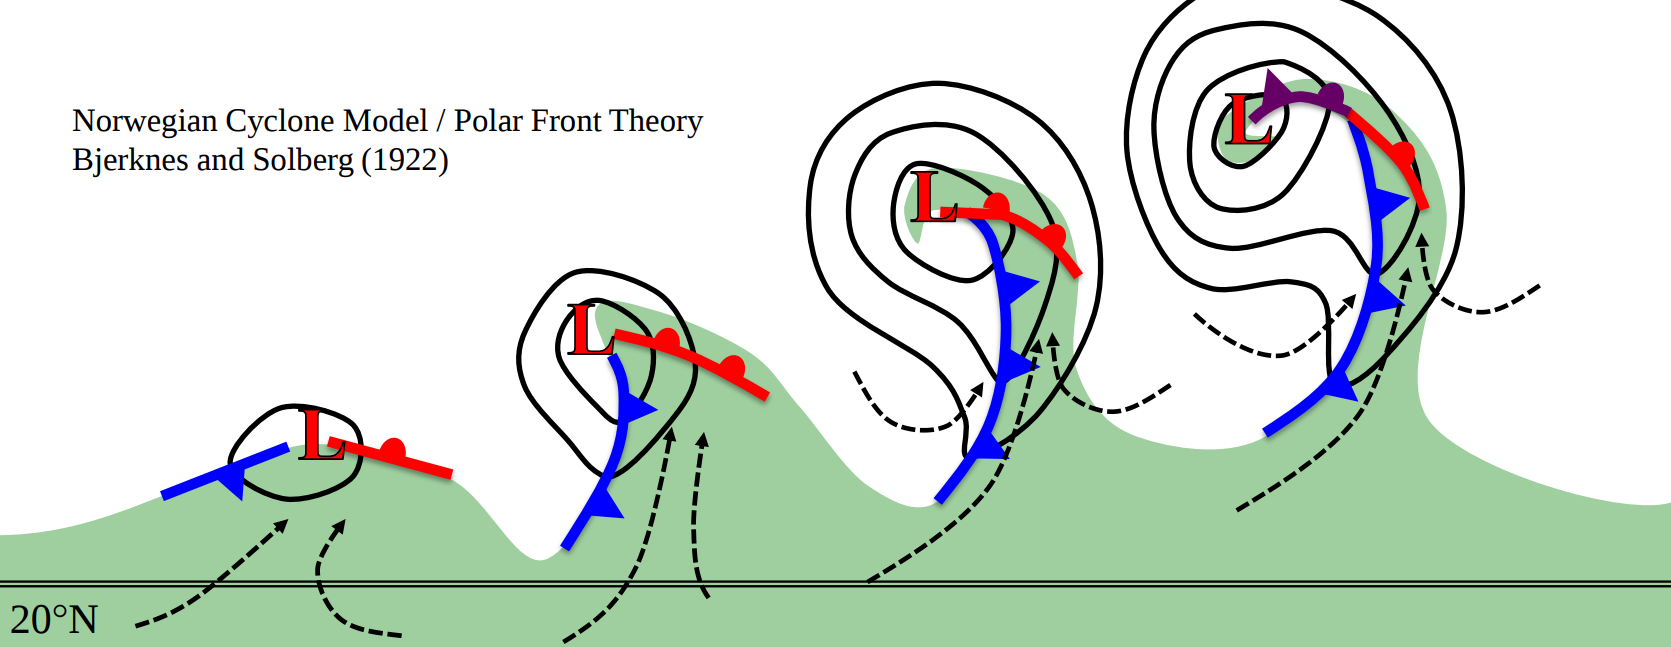
\includegraphics[width=0.8\textwidth]{Arformation.png}
    \caption{A model of co-occurring cyclogenesis and AR formation. This was clipped (and text was adapted) from a presentation made by Dr. Jason Cordeira \cite{Cordeira2016Mid-LatitudeRivers} at the 2016 International Atmospheric River Conference in San Diego, California \cite{Ralph2017AtmosphericFocus}. See text for a description.}
    \label{fig:ARformation}
\end{figure}

%\subsection{Climate dynamics and ARs}

% \subsection{Large scale flows and ARs}

\subsection{The Hadley cell and ARs}

The \textit{Hadley cell} (HC) is a thermally direct circulation which initiates in the tropics via deep convection and terminates in the subtropics around 30$^\circ$. We see this action of the HC in annual-mean zonal-mean mass stream function plots. When we stratify zonal-mean stream function plots by season (see Grotjahn, 1998, pp. 68-69), we see an important component of seasonality: the boreal winter HC shifts equatorward and strengthens considerably in terms of mass flux, ascending south of the equator and descending at 30$^\circ$N; meanwhile, the boreal summer HC shifts poleward and weakens considerably, ascending north of the equator and descending closer to 40$^\circ$N. High pressure ridges produced by the descending branch lead to the generally dry, hot, and stable conditions which characterize the subtropics. 

These conditions can provide controls on AR activity. For one, strong stability in subsiding regions can depress baroclinic growth rates, inhibiting the formation of ETCs and by extension, ARs. Evidence for this is shown best by maps of ETC storm track density (e.g., \cite{Dacre2009TheCyclones}) and AR occurrence frequency (e.g., \cite{Guan2017}), both of which show little activity equatorward of 30$^\circ$. We note as well that seasonal maps of AR frequency occurrence show expected latitudinal shifts, wherein winter ARs occur further equatorward than summer ARs \cite{Kamae2017AtmosphericVariability}. Additionally, evidence suggests that subsidence related to the HC can affect AR moisture transport by blocking the warm sector of an ETC from connecting with the concentrated (sub)tropical moisture source region. This reduces the poleward advection of low-latitude moisture performed by ARs, potentially resulting in ARs fueled more by local MFC rather than long-distance transport \cite{Bao2006InterpretationMoisture}. 
\subsection{Jet streams and ARs}

Westerly upper-tropospheric jet streams provide steering flows for ARs and can have profound impacts on AR activity. Two dominant jet streams exist: 1. the subtropical jet (STJ), which is thermally driven and tends to exist at the poleward flank of the HC; and 2. The Polar Front Jet (PFJ), which is eddy driven, and tends to exist along the polar front. The meridional spacing between these jets implies 

% The midlatitude baroclinic zone tends to exist just north of the HC terminus, at approximately 30-60$^\circ$. This zone, rather than being dominated by the action of a large meridional cell, is instead characterized by the mean activity of baroclinic eddies. These eddies advect warm tropical air poleward, and cold polar air equatorward, acting to decrease the meridional temperature gradient. Furthermore, the eddies tend to develop a tilt in their axes leading to the poleward advection of westerly momentum flux (\cite{Grotjahn}, pp. 108). This momentum flux converges in the midlatitudes and forms the eddy-driven jet, sometimes called the polar front jet (PFJ), due to its location along the polar front. 

% We can broadly define two modes for the PFJ, both of which are shown in Fig. \ref{}. We see in the left event, E1, that the AR is attended by a deep trough reaching into the (sub)tropical moisture reservoir. This is in contrast to the right panel, E2, which shows a comparatively more zonal orientation \footnote{Hereafter when we say ``zonal'' orientation or flow, we mean that the wave has little meridional amplitude. By contrast, a ``meridional'' flow is one which meanders and exhibits more exaggerated ridges and troughs.} in the flow pattern.

% From these simple schematics alone, we can imagine the consequences of synoptic flow patterns on AR vapor transport. First, given the plunging trough to its west, the AR in E1 appears to directly ``tap'' into the (sub)tropical moisture reservoir, while the AR in E2 does not. Perhaps then, E1-ARs will have higher vapor content originating from the (sub)tropics, and the vapor in E2-ARs will have a larger contribution from local frontal MFC. We can furthermore suppose that 
% E1-ARs will have higher IWV overall, since the warm (sub)tropical region has the highest concentration of atmospheric water vapor in the world. 

% In addition to moisture origin, we might also suspect that Rossby wave activity can modulate ultimate termination point of an AR. second, E1-ARs might advect more vapor poleward than E2-ARs, as the predominantly zonal flow in E2 directs the AR eastward, while the meridional flow of E1 steers the flow poleward.

% Of course, Fig. \ref{} is a schematic only, and while the suppositions presented may have some physical intuition behind them, the real world often proves a much more complicated place. When it comes to the first point, we note that a climatology of Eastern Pacific ARs performed by \cite{Payne2014DynamicsReanalysis} found that ARs in general were strongly associated with AWB, with the most extreme subset of ARs---defined by the 90th percentile of IVT---occurring with the AWB region on the equatorward side of the AR. This suggests that the large-scale flows associated with AWB-ARs are favorable not just to ARs in general, but to particularly strong AR events. We note further that an observational case study by \cite{Ralph2011} did in fact find that upper-level characteristics similar to those shown in our AWB schematic---specifically, a positively tilted, deep trough to the west of an AR---allowed an AR to directly tap into the tropical moisture reservoir, suggesting that perhaps the flow patterns surrounding AWB may also allow a direct conduit to this region of concentrated IWV. 

%\subsubsection{Rossby waves and ARs}

%As discussed earlier in our brief QG analysis, Rossby waves have important interactions with surface cyclones. Evidence is mounting for AR--Rossby wave interactions as well. In particular, Rossby wave breaking (RWB)---characterized by the rapid (taking place on the order of one day), irreversible overturning of PV contours on an isentropic surface---appears to have important consequences for ARs. We can see this distinctly as a reversal in the meridional PV gradient on an isentropic surface (see Fig. \ref{} for an illustration)

%Rossby waves (RWs) are large scale %\footnote{Large enough that the \textit{Beta effect}, or the meridional gradient of planetary vorticity, is non-negligible. This gives us wavelengths $\mathcal{O}(1000 \textrm{km})$, or $Ro << 1$, where $Ro = \frac{1}{fT}$ is the Rossby number, $f$ is Coriolis parameter, and $T$ is the timescale of the disturbance in question. In words, a Rossby wave has a lifetime of at least }
%meanders in the mean flow which propagate against the Earth's background vorticity gradient (which is caused both by the spherical shape of the planet as well as surface height differences induced by topography). By modulating flow throughout the tropospheric column, RWs influence surface weather including ARs.  %Ignoring these surface height differences and recalling that planetary vorticity $f=2 \Omega \sin(\phi)$, where $\Omega$ is the rotation rate of the Earth and $\phi$ is latitude in radians, we conclude that $f$ increases with increasing latitude. Similarly, PV increases with latitude as well. If we were to examine PV on an isentropic surface, say 350K, we would further see that this surface roughly correponds to the tropical tropopause and the extratropical lower stratosphere. Since stratospheric air has exceptionally high PV due to its strong static stability, the planet has a positive background poleward PV gradient. Generally speaking, we would see the same positive meridional PV gradient embedded within Rossby waves. 
%However, just as ocean waves break, so too can Rossby waves. According to \cite{McIntyreandPalmer} \textit{Rossby wave breaking} (RWB) occurs when there is a rapid (taking place on the order of one day), irreversible overturning of material contours. We can see this distinctly as a reversal in the meridional PV gradient on an isentropic surface (see Fig. \ref{} for an illustration). Two distinct classifications of RWB are examined in the literature: anticyclonic RWB (AWB) and cyclonic RWB (CWB), where AWB (CWB) is characterized in the northern hemisphere as having a southwest-northeast (southeast-northwest) trough tilt (e.g., \cite{Huetal2017}; (see Fig. \ref{}). 

%By changing the mean flow patterns, we can suppose how an AR influenced synoptically by an AWB event might differ from one influenced by a CWB event. Returning to our lovely Fig. \ref{}, note the colored contours of IWV. First, we see in the AWB event, we have a deep trough reaching into the (sub)tropical moisture reservoir. This is in contrast to the CWB panel, which shows a comparatively more zonal orientation \footnote{Hereafter when we say ``zonal'' orientation or flow, we mean that the wave has little meridional amplitude. By contrast, a ``meridional'' flow is one which meanders and exhibits more exaggerated ridges and troughs.} off the coast. From these schematics alone, we can imagine a couple potential relevant consequences. First, the AR in the AWB event appears to more effectively ``tap'' into the (sub)tropical moisture reservoir; since this warm region has the highest atmospheric water vapor content in the world, we would expect AWB-ARs to transport more moisture overall. Second, CWB-ARs might advect less vapor poleward than AWB-ARs, as the former are steered eastward by the predominantly zonal flow, and the latter are steered poleward by the steep meridional flow. 

\subsection{QG forcing of ARs}

 %With a westerly flow and a wind speed maximum in the center of our diagram, we define the \textit{entrance} region as on the left of the diagram, and the exit as on the right (labeled). We define the rest as if we are following the flow (facing the same way as the geostrophic wind vectors): so now, the poleward side is the left-hand side, and the equatorward side is the right-hand side. This leaves us with four quadrants: the left entrance, right entrance, left exit, and right exit regions (labeled). We note that between the left entrance and exit regions, there exists a positive vorticity maximum at the minimum of the embedded trough; similarly, a negative vorticity maximum exists between the right entrance and exit regions at the maximum of the embedded ridge. Thus, we have maximum PVA (and therefore, $\chi < 0$; see Eq. \ref{eq:qualHeightTendency}) at the right entrance and left exit regions of the jet streak, leading to synoptic scale ascent in these quadrants. Conversely, we have maximum NVA ($\chi>0$) and therefore subsidence in the left entrance and right exit quadrants of the jet streak. 

The QG system of equations can provide us with a useful framework for describing the synoptic scale dynamical processes behind AR vapor uptake. Consider an upper-level \textit{jet streak}, that is, a local wind speed maximum embedded in the jet stream, 
% Maximum PVA at the right entrance and left exit regions leads to divergence aloft, thereby leading to mass loss in the column below those regions. Surface air must replace this mass, leading to low-level convergence and rising motions. By contrast, the left entrance and right exit regions feature maximum NVA and convergence aloft, and so lead to sinking motions. 
that moves over an AR propagating over the ocean surface. If the AR is positioned beneath a region of upper-level ascent in the jet streak, MFC in the column and the uptake of water vapor will be favored, strengthening the AR \cite{Cordeira2013The2010}. Conversely, the AR may find itself beneath a column of sinking air related to upper-level convergence in the jet streak. This situation instead favors low-level moisture flux \textit{divergence} and may thereby weaken the AR.

The influence of jet streaks does not end at AR vapor uptake or loss, as QG forcing also has implications for AR precipitation. In particular, we focus on how QG processes can add to or take away from AR orographic precipitation.\footnote{We discuss AR orographic precipitation later, in the Boundary Layer Effects section} %Recall that by QG forcing, upper-level divergence will favor precipitation by enhancing ascent, while upper-level convergence will damp precipitation by weakening ascent. If we take this into consideration we can imagine situations in which upper-level dynamics can either add to or subtract from orographic forcing. 
Say an AR impinges on a mountain barrier while under the influence of a region of upper-level divergence: the forced synoptic scale ascent could intensify the orographic ascent and enhance precipitation further than predicted by orographic lift alone. Conversely, upper-level convergence by a jet streak could oppose orographic lifting, thereby weakening AR overland precipitation by damping upward motions. A QG analysis on US west coast precipitating ARs had such results \cite{HechtCharacterizingCalifornia}.
% performed a QG analysis on US west coast precipitating ARs. The two AR regimes composited had nearly identical landfall locations (controlling for orographic effects) and statistically indistinguishable IVT and IWV. In the first regime, ARs made landfall under the right exit region of a straight jet streak---a region characterized by upper-level convergence. Precipitation in this case was substantially lower than when the AR made landfall under the exit region of a cyclonically curved jet streak, where upper-level divergence dominates. 
The authors noted that QG forcing was one of several factors influencing AR precipitation. Nevertheless, they (and we) maintain that it was this confluence of factors---rather than an isolation of one or another---which enhanced AR precipitation so greatly, and assert that results such as these emphasize the three-dimensional nature of the dynamics which impact ARs. 



%As an AR makes landfall, its orientation with respect to local topography can influence precipitation. Forced ascent of moist air by a mountain range in general enhances precipitation, and the upslope wind component tells us how much of the wind travels directly up the mountainside. Thus, the upslope component of the wind---that is, the wind component normal to the mountain slope---impacts the magnitude of orographic ascent. By Figure \ref{fig:waves} we can see how AR orientation can affect the upslope component of the AR's winds. Suppose S1 hits a coastal mountain nearly perpendicular to its slope, whereas S2 hits at an acute angle. In such a case we would expect the most orographic ascent for S1, and consequently, the highest amount of orographically enhanced precipitation.  

% \subsection{Water in the atmosphere}\label{moist}

% \textbf{The Clausius-Clapeyron (CC) relation:} An equation describing the relationship between temperature and saturation vapor pressure (denoted $e_s$), or the maximum partial pressure water vapor can exert on its surroundings before condensing. For meteorological purposes, the following simplification of this differential equation is often used: $e_s(T) = 6.1094\exp\big(\frac{17.625T}{T+243.04}\big)$, where $T$ is temperature in degrees Celsius. 

% \textbf{Specific humidity ($q$):} The mass of water vapor per mass of air.  For convenience, we often discuss the \textit{saturation specific humidity}, $q_s$, the maximum mass of water vapor a given mass of air can ``hold'', in lieu of $e_s$. When $q = q_s$ within a parcel of air, that parcel is said to be \textit{saturated}. By the CC relation, when using $T$ values typical of the troposphere, we can expect an approximate increase in $q_s$ of 6-8\% per 1 K temperature increase. 

% \textbf{LH} (of water): The energy associated with phase changes of water. For instance, evaporation involves water moving from a lower-energy state of matter (liquid) to a higher-energy one (gas). Thus, we describe evaporation as a cooling process, as it requires an input of energy from the environment to occur. The opposite process, condensation, then represents a heating process, as it releases energy into the environment. This concept emphasizes that water vapor transport represents not just a transport of mass, but of energy as well. 

% \textbf{Scale height ($H$):} The height over which some quantity decreases by a factor of $e$. The $H$ of air (vapor) is given by: $H_{(v)} = \frac{R_{(v)}T}{m_{(v)}g}$, where $R$ is the gas constant for dry air (water vapor) and $m$ is the molar mass of air (water vapor). When we plug in relevant constants and typical tropospheric temperatures, we get $H_{air} \approx 8$ km and $H_{vapor} \approx 2$ km. 

% \subsection{Atmospheric (in)stability}\label{stab}

% \textbf{Lapse rate of the environment:} The change in air temperature with height $(\frac{dT}{dz} = \Gamma)$. In general throughout the troposphere, $\Gamma < 0$ (temperature decreases with height). Environmental lapse rates (ELR) are not fixed, and vary by location, time of day, and environmental conditions.  

% \textbf{Lapse rates of parcels:} The change in temperature an air parcel experiences with changes in altitude. An unsaturated parcel of air will experience the \textit{dry adiabatic lapse rate}, $\Gamma_d = 9.8$ K km$^{-1}$ as it rises (adiabatic cooling) or falls (adiabatic warming). By contrast, a saturated parcel of air's temperature will change at the \textit{saturated adiabatic lapse rate}, often reported as $\Gamma_s = 5$ K km$^{-1}$. Since $q_s$ varies with temperature, a parcel of air may reach or leave saturation as it rises or falls, causing a change in that parcel's lapse rate. When an unsaturated parcel cools enough to reach saturation and then force its moisture to condense, we say that it has reached its \textit{dew point temperature} and we call this height in the atmosphere the \textit{lifted condensation level.}

% \textbf{Potential temperature $(\theta)$:} The temperature a parcel of air originating from some arbitrary pressure level $P$ would attain if brought adiabatically to a standard reference pressure $P_0$, usually 1000 hPa. Like potential energy increases with height, so does $\theta$ (with caveats---see Table 1). Furthermore, since $\theta$ is a conserved quantity, a parcel's $\theta$ will remain the same even as the parcel's altitude changes. As parcels ascend and descend, they follow lines of constant $\theta$, called \textit{isentropes} (as in, lines of constant entropy). 

% \textbf{Virtual [potential] temperature $(T_v, [\theta_v])$:} A measure of [potential] temperature which includes diabatic effects associated with water (e.g., the water in a parcel as it descends will provide some compensating evaporative cooling to the adiabatic warming).  

% \textbf{Static stability:} A property of atmospheric thermal stratification and its ability to damp vertical motions. One measure of this is the dry (moist) \textit{Brunt-Vaisala (BV) frequency squared}, given by $N_{(m)}^2 = \frac{g}{\theta_{(v)}}\frac{\partial \theta_{(v)}}{\partial z}$. It describes the buoyancy oscillation a parcel of air will undergo if perturbed under dry (moist) stable environmental conditions. Table 1 describes different (in)stability scenarios and the thermal stratification associated with them. 

% \begin{table}[h]\label{tab:stab}
% \resizebox{\textwidth}{!}{
% \begin{tabular}{P{2.5cm} | P{6cm} | P{2.5cm} | P{2.2cm} | P{2cm} }
% Scenario & Parcel response to displacement &  ELR ($\Gamma$) & $\theta$ lapse rate & BV freq. \\ \hline
% Stable & Attempt return to initial position, then oscillate with frequency $N_{(m)}^2$. & $\Gamma_{(m)} < \Gamma_{d(s)}$ & $\frac{\partial\theta_{(v)}}{\partial z} > 0$ & $N_{(m)}^2 > 0$ \\ 
% Neutral & Will remain in new position. & $\Gamma_{(m)} < \Gamma_{d(s)}$ & $\frac{\partial\theta_{(v)}}{\partial z} = 0$ & $N_{(m)}^2 = 0$ \\
% Absolutely unstable & Will overshoot perturbation until equilibrium temperature is reached. Note: occurs whether parcel is dry or saturated. & $\Gamma_{(m)} > \Gamma_d$ & $\frac{\partial\theta_{(v)}}{\partial z} < 0$ & $N_{(m)}^2 < 0$  \\
% Conditionally unstable & Will overshoot perturbation \textit{as long as the parcel is saturated.} & $\Gamma_d > \Gamma_m > \Gamma_s$ & $\frac{\partial\theta_v}{\partial z} < 0$ & $N_m^2 < 0$   \\
% \end{tabular} } 
% \caption[Table caption text]{Summary of dry and moist (when applicable) static stability scenarios. Subscript m denotes moist variables (or in the case of $\Gamma_m$, that the parcel is saturated), while (v) denotes the use of virtual temperature correction.}

% \end{table}

\section{Thermodynamics of ARs}\label{sec:thermoAR}

% While large-scale dynamics plays its part in dictating AR moisture origin and transport, thermodynamics places important constraints on the water vapor content of the atmosphere itself. %Horizontal maps (\ref{fig:hq}) and vertical distributions (\ref{fig:vq}) of $q$ conveniently illustrate the relationship between atmospheric temperature and vapor content. Note the concentrated ribbon of water vapor over the tropics, as well as the ARs branching from that ribbon into the midlatitudes. Images like this gave rise to the term \textit{atmospheric river} itself, as ARs appear to directly tap into tropical moisture. Of course, as already described, the story is not quite that simple.
% We will build on Section \ref{sec:synAR} here by including a discussion of the \textit{thermo}dynamic modulation of AR water vapor content and precipitation. 

\subsection{Temperature controls on AR vapor}

Our discussion of AR moisture begins with the \textit{Clausius-Clapeyron relation}, which describes the relationship between temperature and saturation vapor pressure. CC partially modulates the availability of water vapor for an AR to sweep up as it propagates along the ocean surface (note: as a surface flux, we will discuss this in more detail in Section \ref{sec:BLAR}). Specifically, \textit{CC-scaling}---the percent increase of saturation vapor pressure per degree temperature increase---is estimated to be about 7\% at typical tropospheric temperatures.\footnote{Note that we say ``about'' $7\%K^{-1}$ because a reference temperature dependency exists in the CC relation. For instance, for an increase of $1K$, the CC relation gives us scaling of $\sim 6\%$ at $T=300K$ and of $\sim 7.4\%$ at $T=270K$.} Since the vapor availability for ARs is ultimately driven by evaporation from the ocean surface, we expect that higher sea-surface temperatures (SSTs) will result in ARs with higher IWV. 

We can see support for our proposed SST--AR IWV relationship in a couple different experimental settings. We note first that subtropical ARs tend to have higher IWV than midlatitude ARs \cite{Ralph2017DropsondeRivers}, which is consistent with predictions from the CC relation given that lower latitudes tend to be warmer. Climate change studies further highlight the role of CC in modulating AR IWV. For instance, ARs simulated under the RCP8.5 scenario---characterized by the largest surface warming by end-of-century for all climate scenarios---experience enough systematic moistening (IWV increase) to increase their IVT despite decreasing AR wind speeds \cite{Payne2015}. Another study examined the moistening response of ARs to near-surface air temperature warming with respect to CC scaling in an RCP8.5 scenario \cite{Gao2015}. It was found that AR IWV actually experienced \textit{super}-CC scaling. In other words, CC scaling under-predicted the actual moistening rate of ARs. The results of this study agreed with the previous that AR IVT gets more intense in a warmer world by the increase in available moisture, in spite of decreasing AR wind speeds. Such results indicate the strong thermodynamic controls on AR moisture transport.  

%Incidentally, CC arguments also show us how cold tropospheric temperatures can weaken an AR and lead to moisture loss. Consider an AR encountering a particularly cold region of air: if the temperature of this air is at or below the dew point temperature of the AR, some of the AR's moisture will condense out, releasing LH to the surroundings. In this manner, ARs can provide substantial LH to the cold high latitudes, even in the absence of actual AR precipitation. This also shows us how an AR can maintain a temperature higher than its surroundings for some time. 


\subsection{Static stability in ARs}

Static stability measures the resistance to vertical motions brought about by the thermal stratification of the atmosphere. In dry air, this is often measured by change of potential temperature, $\theta$, with height. The Brunt-V\"ais\"al\"a (BV) frequency squared ($N^2$) is proportional to the vertical stratification of $\theta$. In general, when $N^2 > 0$ ($\theta$ increases with height) we have a stable atmosphere which resists vertical motions; when $N^2 < 0$, we have an unstable atmosphere in which convective overturning may occur spontaneously; and when $N^2 = 0$, we have a neutral atmosphere which does not resist perturbations. However, a funny thing happens in saturated conditions: as a parcel ascends, the LHR associated with condensation partially compensates for adiabatic cooling. In such a case, $N^2$ as formulated for a dry atmosphere tends to be too small  \cite{Durran1982OnFrequency}. 

Since we are concerned with the density difference between parcel and atmosphere, perhaps we should instead use the \textit{virtual potential temperature}, $\theta_v$, which accounts for the presence of water vapor on the density of a given mass of air. We need an additional correction for moisture due to LH release on condensation: the \textit{equivalent potential temperature}, $\theta_e$, remains constant for a parcel even if all its moisture condenses and its LH is released. Unfortunately, we cannot simply substitute some combination of $\theta_v$ and $\theta_e$ for $\theta$ to find a moist BV frequency. The moist BV frequency squared, $N_m^2$, is quite a bit more complicated than that \cite{Durran1982OnFrequency}, and describing its derivation is well outside the scope of this document. 

We turn our attention now to describing AR stability in terms of $N^2$, $N_m^2$, and the vertical distribution of $\theta_e$. A case study of an AR \cite{Neiman2008MeteorologicalObservations} found dry static stability ($N^2 > 0$; $\frac{\partial\theta_e}{\partial z} > 0$) throughout the column, including in the lowest 2 km layer. This AR impinged on a mountain range with a height of approximately 1 km. Given the stable conditions indicated by $N^2$, we would expect some resistance to orographic uplift, potentially limiting the AR's ultimate precipitation. However, the near-saturated conditions of the AR make $N_m^2$ a better predictor of layer instability. Consistent with the devastating precipitation produced by the AR, it was found that $N_m^2 \sim 0$ ($\frac{\partial\theta_e}{\partial z} \sim 0$) throughout the column, with $N_m^2 < 0$ ($\frac{\partial\theta_e}{\partial z} > 0$) in the lowest 1 km. The authors of the case study noted that this potential instability within the lowest layer, coupled with the moist-neutral conditions aloft, were ``highly conducive to orographic precipitation enhancement'', at least from a thermodynamic perspective.  
% Thermal structure has further impacts in the ultimate hydrologic consequences of AR precipitation. As one could imagine, a cold AR favors frozen precipitation and can provide substantial snowpack. Conversely, an AR which originated over warm tropical waters or has experienced sufficient warming by LH can remain at above-freezing temperatures despite adiabatic cooling while ascending over a mountain. In such a case, not only can high altitudes receive rainfall, but that rainfall can result in particularly destructive rain-on-snow events (ROSs). ROSs can lead to devastating floods not just because the rain itself runs off the snow, but because the LH released by the rain raises near-surface temperatures and melts existing snowpack. %Such events show the sensitivity of AR impacts to temperature.

\subsection{Thermodynamic feedbacks between ARs and ETCs}\label{sec:ARsandETCs}
% Whether one ascribes to the AR formation model of D15 or the one summarized in Section \ref{sec:M2}, a clear dynamical link exists between ARs and ETCs, even if the precise cause-and-effect relationship still contains mysteries. ETCs can pretty directly influence the formation and maintenance of ARs, but what about the other way around? As a part of our model, we glossed over this idea that ARs can strengthen ETCs in Step 2. Here we discuss some evidence for LH (and ARs) in strengthening ETCs
% \subsubsection{How LH can provide ``fuel'' for ETCs}

% The quasigeostrophic (QG) system of equations provides a convenient framework for describing how LH can intensify surface cyclogenesis. When deriving the QG height tendency ($\chi$) and vertical velocity ($\omega$) equations in synoptic dynamics classes, we tend to ignore the diabatic heating term in the thermodynamic equation; however, if we do decide to keep it, these equations (qualitatively) take the following forms in an isobaric coordinate system: 
% \begin{equation}\label{eq:qualHeightTendency}
% \chi = -\textrm{(absolute vorticity advection)} + \frac{\partial}{\partial p} \textrm{(thermal advection)} + \frac{\partial}{\partial p} \textrm{(diabatic heating)}
% \end{equation}
% \begin{equation}\label{eq:qualOmega}
% \omega = \frac{\partial}{\partial p} \textrm{(absolute vorticity advection)} - \textrm{(thermal advection)} - \textrm{(diabatic heating)}
% \end{equation}
% where $\frac{\partial}{\partial P}$ denotes the vertical differential of the term. 

% We now use these ``equations'' to illustrate cyclogenesis from a QG perspective. Figure x shows a surface cyclone (with attendant WCB) and 500 hPa trough in a configuration favorable for cyclone deepening. Why is this? Consider the following (very brief) assessment, where the diabatic (moist) effects are printed in \color{blue}blue \color{black} to visually separate them from dry dynamics: 
% \begin{itemize}\setlength\itemsep{0em}
% \item[A.] Negative vorticity advection (NVA) is maximized aloft and 0 at the surface here (note that a surface high is a local minimum in vorticity). Thus we have $\chi > 0$ (rising heights) and $\omega > 0$ (sinking air). Sinking air increases column air mass and strengthens the surface high. 
% \item[B.] Cold air advection (CAA) is maximized at the surface cold front and very small aloft; thus we have $\chi < 0$ (falling) and  $\omega > 0$, deepening the trough despite small opposition by adiabatic warming. 
% \item[C.] Maximum positive vorticity advection (PVA) aloft leads to $\chi < 0$ and $\omega < 0$ (rising motion). This rising motion lowers column air mass above the surface low, intensifying it. 
% \item[D.] Warm air advection (WAA) by the surface warm front causes $\chi > 0$ (assuming WAA decreases with height) and $\omega < 0$. \color{blue} In addition, maximum diabatic heating at 500 hPa occurs due to ascent of moist air in the WCB, again giving us $\chi > 0$. Like WAA, this diabatic heating also leads to $\omega < 0$. In short, these diabatic effects allow the ridge to build further than if we looked at dry dynamics alone in our idealized case. \color{black}  The ridge builds despite slight opposition from adiabatic cooling as the air rises.
% \end{itemize}
% How exactly does building a ridge enhance a surface cyclone? To answer this question most simply, we focus on potential vorticity (PV): 
% \begin{itemize}\setlength\itemsep{0em}
%     \item[1. ]As the ridge height increases, the resulting thickness increase of the 1000--500 hPa layer stretches the column of air. By PV conservation, the increased depth of the column must increase the relative vorticity, $\zeta$, of the column. 
%     \item[2. ]This increased $\zeta$ then enhances the cyclonic circulation in the layer, deepening the surface low further. Enhanced surface convergence drives $\chi > 0$ at 500 hPa and $\omega < 0$ in the 1000--500 hPa layer, further increasing layer thickness. 
%     \item[3. ]The column stretches, causing $\zeta$ to increase, further enhancing the cyclonic circulation, deepening the surface low... etc. 
% \end{itemize}
% We have here a positive feedback loop which illustrates how diabatic heating---in our case, from LH release---in the column can enhance surface cyclogenesis. This feedback loop will continue until some opposition occurs, say if adiabatic cooling from the rising heights offsets the diabatic heating, or if the phase difference between the midlevel wave and surface low enters a configuration less favorable for cyclogenesis.

%Potential vorticity (PV) provides a convenient framework for describing the role of LH in cyclogenesis. Under adiabatic, frictionless, incompressible conditions, a parcel's PV will not change as long as it follows isentropes. Thus, it is a conserved quantity. Therefore, if any of the stated conditions are not met (e.g., diabatic heating is allowed), we have a nonconservation of PV. 

% Above we presented a simple model for how LH release in the WCB might strengthen surface cyclogenesis. Here we move on to very briefly summarize some of the evidence for LH release in enhancing cyclogenesis, as well as emerging evidence on the relationship between ARs and cyclogenesis.

AR moist thermodynamics happens to have consequences for cyclogenesis. In particular, LH release is associated explosive cyclogenesis---sometimes called \textit{bomb cyclogenesis}---which occurs when the surface pressure in an ETC deepens by at least 24 hPa in 24 hours. Hindcasts of ``bomb cyclones'' in a model featuring a dry dynamical core only reached approximately 50\% of the pressure deepening obtained from simulations with moist effects included, while only one of two simulated cyclones experienced explosive deepening from dry effects alone \cite{Reed1988TheForecasts}. Another study attributed 60\% of the deepening in three bomb cyclones to condensation heating \cite{Fink2012DiagnosingAtlantic}. 
% used an original formulation of the pressure tendency equation to diagnose the relative roles of dry baroclinic and moist diabatic contributions to cyclogenesis. They found that three of the five simulated bomb cyclones had approximately , while the deepening of the other two was largely due to dry dynamics. 

If latent heat release plays a role in explosive cyclogenesis, we expect ETCs with attendant ARs to more frequently experience it than those without ARs. Indeed, a recent study of ETC climatology in reanalysis output found that approximately 80\% of bomb cyclones were associated with a nearby AR within six hours of the ETC's maximum deepening rate \cite{Eiras-Barca2018TheBasins}. By contrast, ARs were detected nearby in only about 40\% of the non-explosive cyclone cases. The authors concluded that LH release when a developing ETC encounters an AR provides an important energy source for further deepening. This presents us with an important AR--ETC feedback: while vapor flux convergence associated with frontogenesis in the ETC warm sector can add to AR moisture content, ARs can in turn strengthen nearby or attendant ETCs \cite{Eiras-Barca2018TheBasins}.


%\textbf{Boundary layer height:} The diurnal evolution of the planetary boundary layer (PBL) height is determined largely by the action of rising thermals which overshoot the capping inversion and drive free atmosphere air into the boundary layer, increasing its mass and causing it to deepen. Thus, surface heat fluxes represent a primary mechanism for boundary layer growth. 

% \textbf{Vertical profile of water vapor:} Since the scale height of water vapor on Earth's atmosphere is approximately 2 km, most water vapor in a column exists in the PBL. Due to the well-mixed nature of the PBL, the concentration of water vapor within it does not vary greatly.

% \textbf{Bulk aerodynamic formula (BAF):} A method used to estimate turbulent heat fluxes from the surface through the PBL. Used in BAFs is a \textit{bulk transfer coefficient}, an empirically derived, dimensionless value of proportionality dependent on surface roughness and atmospheric conditions (e.g., stability).  

% \textbf{Surface sensible heat fluxes (SHF):} Turbulence-driven conductive heat flux from the surface of the planet to the atmosphere. The BAF for SHF is proportional to the temperature differential between the surface and a reference height (usually 2 or 10 m), the horizontal wind speed at that height, and the bulk transfer coefficient for the surface.   

% \textbf{Surface LH fluxes (LHF):} Turbulence-driven LH flux (e.g., evaporation) from the surface. For the sea surface, the LHF BAF is similar to that for SHF, but is dependent instead on the difference between the surface $q_s$ and $q$ for the reference height.

% \subsection{Low-level jets}

% \textbf{Low-level jet (LLJ):} A thin ribbon of relatively fast-moving air (approx. 10-40 ms$^{-1}$) usually within the bottom 2 km of the atmosphere. Researchers have documented various LLJ types and formation mechanisms; we summarize two relevant LLJs below. 

% \textbf{Pre-frontal jets:} LLJs can form along fronts, like the pre-cold-frontal LLJ seen in Figure \ref{AR1b}. They form at least in part due to a reversal of the temperature gradient ahead of the cold front (i.e., the thermal wind relationship) \cite{BrowningPardoe}. That said, the diabatic effects of LH release also play a role in raising the near-surface wind speeds (\cite{Lackmann2002}). 

% %\textbf{Coupled jet streaks:} LLJs may form along the surface as a \textit{return circulation} to the transverse circulations induced by convergence and divergence aloft (Figure \ref{fig:jetstreak}, thick red arrows). Being return circulations, the surface winds induced in such a way would flow in the opposite direction (Figure \ref{jetstreak}, thin red arrows) (see pp. 417-419 of \cite{Carlson1998Mid-LatitudeSystems} for more information on jet streaks and induced low-level flows).

% \textbf{Mountain barrier jet:} An LLJ which flows parallel to a mountain range. Consider a cold front blowing in from the west and encountering a north-south mountain range (e.g., the Sierra Nevada Mountains): the upslope wind component must overcome the barrier and ascend over it. Under stably stratified conditions, this westerly wind has a lower potential temperature than the air over the mountains. As it ascends, it brings this potentially colder air over the barrier, inducing a pressure gradient force down the windward side of the mountains. Coriolis acceleration deflects this induced easterly flow northward, leading to a southerly, along-barrier LLJ. 

\section{Boundary layer processes in ARs}\label{sec:BLAR}

% While we have gone over some large-scale dynamical as well as thermodynamical mechanisms behind ARs, the surface evaporation which fuels these systems is a distinctly boundary layer subject. When we couple this with the fact that much of the AR moisture exists within the atmosphere boundary layer (ABL), it should be clear that ABL processes must be included to provide a more complete picture of ARs. 
\subsection{Surface fluxes and ARs}

We begin with the bulk aerodynamic formula (BAF) for LH flux \footnote{}, which parameterizes the turbulent transport of LH and so can help us understand what feeds ARs. The BAF for LHF is positively proportional to the near-surface wind speeds. We hypothesize that the pre-frontal LLJ associated with ARs can contribute to AR moisture by raising along-AR wind speeds and increasing the turbulent transport of water vapor, but we note that we unfortunately could not find any studies which examined this. We could envision a simple case study comparing an AR with attendant LLJ against one without could help elucidate the role, if any, of the LLJ in the turbulent transfer of water vapor into an AR. 

Surface fluxes which impact ARs do not entail only water vapor. Cloud condensation nuclei (CCN) are intensely important for precipitation, since they modulate cloud droplet size and whether ice or liquid cloud drops form. Since ARs are largely oceanic systems and marine air tends to be quite clean, turbulent fluxes of sea spray aerosol (SSA) may have particular significance for ARs. AR or adjacent LLJ wind speeds can raise wave heights, increasing the uptake of SSA. SSA happens to act largely as an ice nucleation particle (INP), a CCN which favors ice formation in mixed-phase clouds. We could not find any published studies on the SSA impacts on AR precipitation, but in one case study, \cite{Ault2011} an AR containing dust (another INP) precipitated substantially more than an AR whose raindrops were found to contain organic compounds. The authors attributed this to the enhanced precipitation efficiency of ice hydrometeors. We note here however that cloud microphysics are sufficiently complex that broadly applying one case study is ill-advised. Nevertheless, we expect that aerosol fluxes from the surface can provide important controls on AR precipitation processes. 

\subsection{Orographic enhancement of AR precipitation}

AR precipitation is often orographically enhanced, that is, influenced by the lift experienced as horizontal flows encounter an orographic barrier (i.e., a mountain range) and are forced over it. At low levels, ARs are sufficiently close to saturation such that the uplift produced by even relatively short mountains can drive orographic precipitation (OP) \cite{Neiman2008MeteorologicalObservations}. 

\subsection{Blocked flows and ARs}

\section{Summary} 

The ``recipe'' for creating an AR has many ingredients, each either enhancing or offsetting another in turn. As we understand it, ARs are dynamically linked with ETCs, but rather than being some inseparable piece of ETC anatomy, ARs represent a 

\section{Quantitative hypotheses on some climate change effects on ARs}

The preceding sections provided nonexhaustive, high-level information on ARs and the synoptic-scale dynamical, thermodynamical, and boundary layer settings and characteristics of them. We now move on from qualitative descriptions to more quantitative ones. In the following subsections, we use fundamental thermodynamics arguments to hypothesize on how climate change might affect AR precipitation. In particular, we focus on thermodynamic constraints set forth by the Clausius-Clapeyron (CC) relation. 

For reference, any experiments mentioned for testing hypotheses will be performed in an aquaplanet global climate model (AQP-GCM). AQP-GCMs feature full-physics atmospheric models with no land, sea ice, or topography---their lower boundary conditions are characterized by ocean cover. In this case, the ocean will provide sea surface temperature (SST) forcing only (i.e., we prescribe it as a lower boundary condition which acts on the atmosphere model, but it is time-invariant and the atmosphere model does not affect the SST in any way). Designing our experiments this way allows us to isolate impacts on ARs as modulated by SSTs alone, and the effects of those SSTs on dynamics and thermodynamics. 

\subsection{Clausius-Clapeyron scaling of AR extreme precipitation} 

We begin here with our master hypothesis (HM): 
\begin{itemize}
    \item[\textbf{HM.}] \textit{Extreme AR precipitation rates will increase linearly with the CC rate of $\sim$ 7\%$K^{-1}$}.
\end{itemize}

For this to work, we describe some basic assumptions. We note they are highly simplified, and will briefly discuss some pitfalls associated with them later. In any case, here we go:
\begin{enumerate}[noitemsep]\vspace{-\topsep}
    \item[A1.] Precipitation rate (P) in a column is constrained by the vertically-integrated condensation rate (C) in the column.
    \item[A2.] Condensation is constrained by relative humidity (RH), that is, how close the layer specific humidity ($q$) is to layer saturation specific humidity ($q_s$). In our model, condensation occurs when $q = q_s$ (at fixed RH). 
    \item[A3.] So, taking A1 and A2 into consideration,
    \begin{equation}
        C \propto - \int_{p_0}^{p_t}q_sdp
    \end{equation} 
    where $p_0$ is the surface pressure and $p_t$ is the pressure at the top of the troposphere. 
    \item[A4.] We assume some \textit{constant fraction}, $\beta$, of condensation falls as precipitation in an AR, giving us
    \begin{equation}\label{Eq:betaC}
        P = \beta C \propto - \beta \int_{p_0}^{p_t}q_sdp
    \end{equation}
    For reference, when it comes to extreme $P$, we expect $\beta \sim 1$, or that all vapor which condenses also precipitates. 
    \item[A5.] Last, we assume that extreme $P$ in general is driven by moisture flux convergence in the column \cite{Trenberth2003ThePrecipitation} and thus is not limited by surface energy constraints on evaporation \cite{Held2006RobustWarming}.
\end{enumerate}
By the (admittedly highly simplified) model given in (\ref{Eq:betaC}), then, we expect AR extreme $P$ (say, 90th, 95th, and 99th percentile; hereafter we refer to AR extreme $P$ to simply as ``AR $P$'' for brevity) to vary with vertically integrated AR $q_s$. 

%We note that our expression for $IWV$ in (\ref{2}) is similar, though using $q$ in place of $q_s$. We use the above assumptions to set $q = q_s$ in a precipitating AR\footnote{Incidentally, ARs tend to be close to saturation anyways \cite{}}. To further simplify things, we set $\beta = 1$; that is, \textbf{our AR precipitation exists within some extreme in which 100\% of the water which condenses also precipitates}. This leaves us with: 
% \begin{equation}\label{eq:AR_IWV}
%     P \propto IWV = - \frac{1}{\rho g} \int^{p_t}_{p_0} q_s dp 
% \end{equation}

% Thus, within our model, variation in AR $P$ is directly related to that in AR IWV. We discuss projected changes in AR IWV next. 

\subsection{CC constraints on AR q}

As described briefly earlier, the CC relation gives us the relationship between equilibrium vapor pressure, $e_s$, and temperature, $T$. By CC, the quantity of vapor above the ocean surface---that is, vapor available for an AR to take up (recall the bulk aerodynamic formula for vapor)---is related to the local SST. Thus, when we discuss changes in $T$ in the context of CC, we mean changes in SST. 

We can use CC to express the fractional change in $\frac{\Delta e_s}{e_s}$ to some $T$ change $\Delta T$: 
\begin{align}\label{eq:ccscale}
    \frac{\Delta e_s}{e_s} = \frac{L\Delta T}{R_vT^2}
\end{align}

What does this mean for AR vapor content? We note that $q_s \propto e_s$, so we can assume $q_s$ scales with $e_s$ and $\frac{\Delta q_s}{q_s} = \frac{\Delta e_s}{e_s}$. Thus, we also expect $\frac{\Delta q_s}{q_s} \sim 7\%K^{-1}$, or a 7\% increase in $q_s$ for each increase per $K$ in SST. 

We bring in yet another simplification to streamline things:
\begin{enumerate}
    \item[A6.] In our model, virtually all of the water vapor in an AR exists within the atmospheric boundary layer (ABL).
\end{enumerate}
We therefore can parameterize the IWV of an AR as
\begin{align}\label{eq:ARq1}
    IWV_{AR} = - \int_{Z_s}^{Z_b} q_{AR} dz
\end{align}
where $Z_s$ is the height of the surface and $Z_b$ is the height of the ABL. When we recall further that turbulent mixing in the ABL results in a relatively steady $q$ throughout, we can treat $q_{AR}$ as a constant and take it out of our integral:
\begin{align}\label{eq:Q_AR}
    IWV_{AR} = q_{AR} Z_{ABL}
\end{align}
where $Z_{ABL}$ is the depth of the ABL. 

Applying product rule gives us: 
\begin{align}\label{eq:Q_AR}
    \frac{\Delta IWV_{AR}}{IWV_{AR}} = \frac{\Delta q_{AR}}{q_{AR}} + \frac{\Delta Z_{ABL}}{Z_{ABL}}
\end{align}

How do we apply this to $P$? We note here that $q_{AR}$ does not always equal $q_s(SST)$; that is, ARs are not always at saturation with respect to SST. However, within a moist marine boundary layer, SST will drive surface fluxes and provide an upper limit on the vapor content of the air (recall the BAF for LH flux). Thus, we assume that any changes in $q_{AR}$ can be attributed to changes in $q_s(SST)$. We also assume here that our $C$ to $P$ conversion ratio, $\beta$, does not change. This leaves us with the following expression and hypothesis: 
\begin{align}\label{eq:QsandP}
    \frac{\Delta P}P \sim \frac{\Delta q_s}{q_s} + \frac{\Delta Z_{ABL}}{Z_{ABL}}
\end{align}
\begin{itemize}
    \item[H1.] \textit{AR precipitation rate will scale linearly with the CC rate as driven by changes in AR $q_s$.} 
\end{itemize}
In other words, for some increase in SST, we expect a CC-predicted increase in $q_s$. Increased column-integrated $q_s$ will drive increases in $C$, in turn driving increases in $P$. Briefly, testing this hypothesis might involve the following steps: 
\begin{enumerate}[noitemsep]
    \item Simulate 2 scenarios which differ by SST (one featuring a globally uniform increase in SST, say +3K, is simplest).
    \item Compare midlatitude mean AR $P$ in both scenarios.
    \item Compare meridional distributions of zonal mean AR $P$ as well to account for spatial variability in response.
    \item If AR $P$ in the +3K uniform scenario is $\sim 21\%$ higher than in the lower-SST scenario, our hypothesis is supported. 
\end{enumerate}
What if our hypothesis is not supported? What if AR P in our simulations scales at a sub-CC or even super-CC rate? We begin a discussion of some mediating factors below. 

\subsection{Factor 1: mean ABL depth might change}

We recall that our model of AR P is related not only to $q_s$, but also AR (or rather, ABL) depth (recall Eq. \ref{eq:QsandP}). We note that in (\ref{eq:QsandP}), if we assume $\frac{\Delta q_s}{q_s} = 0.21$ (remember, we are using a +3K uniform warming scenario here), then:
\begin{align}\label{eq:QsPABL}
    \frac{\Delta P}{P} - 0.21 \sim \frac{\Delta Z_{ABL}}{Z_{ABL}}
\end{align}
This leads us to:
\begin{itemize}
    \item[H2.] \textit{Departures from the CC rate in AR P are driven by changes in ABL depth.}
\end{itemize}
Two scenarios pop up here: 
\begin{enumerate}
    \item If $\frac{\Delta P}{P} < 0.21$, we expect here that $\frac{\Delta Z_{ABL}}{Z_{ABL}} < 0$, or a shallower ABL.
    \item  If $\frac{\Delta P}{P} > 0.21$, we expect here that $\frac{\Delta Z_{ABL}}{Z_{ABL}} > 0$, or a deeper ABL. \footnote{Incidentally, we hypothesize that a deeper ABL may help explain the super-CC scaling of AR moisture \cite{Gao2015}.}
\end{enumerate}
Testing this hypothesis is a bit more complicated than testing H1, because ABL depth can be difficult to determine. Fortunately, climate models can output ABL depth, so we could always compare mean ABL depth model outputs during AR conditions across our simulations. 

If the values found for $\Delta Z_{ABL}/Z_{ABL}$ satisfy (\ref{eq:QsPABL}), then H2 is supported, and we can indeed ascribe departures in AR P from the CC rate to changes in ABL depth. However, if our findings for $\Delta Z_{ABL}/Z_{ABL}$ (for instance, maybe ABL depth does not change; or maybe it does not change enough to account for observed changes in $P$) do not provide closure for our simple equation, we will have to introduce further modulating factors. 

\subsection{Factor 2: we need to include some dynamics (wind)!}

Recall that ARs are characterized as systems of enhanced vapor \textit{transport}, with their vapor transport often quantified by IVT (\ref{1}). Since extreme precipitation is often related to low-level moisture flux convergence \cite{Trenberth2003ThePrecipitation}, then low-level wind speeds within an AR may provide a missing piece in the AR $P$ vs. CC puzzle.

While we can pretty confidently assume that $q_s$ within the ABL does not change with height, we cannot do the same for horizontal wind speed, $U$. Instead we assume it follows a logarithmic profile, or perhaps we have a LLJ as documented in the AR literature (recall Fig. \ref{AR1b}). In any case, we define some AR-mean $U$ within the ABL as $\overline{U}$. We can now define $IVT_{AR}$ as: 
\begin{align}\label{eq:ArIVT}
    IVT_{AR} = \overline{U}\times(RH\times q_s \Delta Z_{ABL})
\end{align}
Or the product of the mean wind and $IWV_{AR}$. 
What could this mean for $P$? Again, we assume that changes in $q_s(SST)$ explain changes in $q_{AR}$, so we substitute $q_{AR} = q_s$. With this in mind, and by using product rule, we get our fractional change in AR $P$: 
\begin{align}\label{eq:IVTandP}
    \frac{\Delta P}P \sim \frac{\Delta \overline{U}}{\overline{U}} + \frac{\Delta q_s}{q_s} + \frac{\Delta Z_{ABL}}{Z_{ABL}}
\end{align}

By (\ref{eq:IVTandP}), we need to account for changes in AR mean wind speeds as well as those in $q_s$ and ABL height. Let us say we have some residual, $r$, from (\ref{eq:QsPABL}); in this case, we have  
% \begin{align}\label{eq:ResQsPABL}
%     \frac{\Delta P}{P} - 0.21 - \frac{\Delta Z_{ABL}}{Z_{ABL}} \sim r
% \end{align}
% By the model presented in (\ref{eq:IVTandP}), we have 
$r = \frac{\Delta \overline{U}}{\overline{U}}$. This leads us to the following equation and hypothesis:
\begin{align}\label{eq:ResQsPABLU}
    \frac{\Delta P}{P} - 0.21 - \frac{\Delta Z_{ABL}}{Z_{ABL}} \sim \frac{\Delta \overline{U}}{\overline{U}} = r
\end{align}
\begin{itemize}
    \item[H3.] \textit{Departures from the CC rate in AR $P$ (not accounted for by ABL depth changes) are related to changes in AR mean wind speeds.}
\end{itemize}
To test H3, we will attempt to balance (\ref{eq:ResQsPABLU}) by calculating fractional changes in AR mean wind speed. To define AR mean wind speed, we could calculate the weighted vertical mean horizontal wind vector magnitude for each simulation and compare them. This could include both AR lifetime mean wind speeds, as well as mean wind speeds during precipitation and extreme precipitation. As with our ABL tests, this gives us two distinct scenarios: 
\begin{enumerate}
    \item If $r>0$, then by our latest model, we expect $\frac{\Delta \overline{U}}{\overline{U}} > 0$, or a strengthening of mean AR wind speed. Increasing AR mean wind speed could lead to enhanced low-level moisture flux convergence, bringing more vapor into the precipitating column. This could help to account for say, super-CC scaling in AR $P$. 
    \item If $r<0$, then we expect $\frac{\Delta \overline{U}}{\overline{U}} < 0$, or a weakening of mean AR wind speed. This could help to account for sub-CC scaling in AR $P$, since damped winds could in turn damp low-level moisture flux convergence.
\end{enumerate}
Again, we hope here to balance our precipitation budget. If we find that this closes our budget (or brings us closer to closure), then our results indicate that AR saturated vapor \textit{flux}, not AR saturated vapor content, is a better predictor of AR $P$, at least in the context of our AQP-GCM simulations. We discuss some potential missing factors and other caveats next, though we begin with a fun thought experiment on how we might use our AQP-GCM to predict AR orographic precipitation.  

\subsection{Factor 3: what about orography?}

AR orographic precipitation---some of the most extreme examples of AR precipitation in the world---is related most directly to the upslope component of the vapor flux. In our AQP-GCM setup, of course, we do not have topography and thus have no way of capturing orographically enhanced precipitation\footnote{We note here that even if we did run experiments in a GCM with terrain, the degree to which we capture orographic precipitation would be a function largely of horizontal resolution (to simulate grid-scale moisture flux convergence against orographic barriers), so we argue that a comprehensive climate model still has its own set of limits in estimating orographic precipitation}. However, the AQP-GCM will include potential changes in Rossby wave meridional amplitude or shifts in the jet streams, and we can use statistical relationships to infer how a 3K SST increase might impact AR orographic precipitation. 

We do this by using the formulation found by \cite{Cordeira2013The2010}:
\begin{align}\label{eq:UpslopeFlows}
    P \propto U_\bot \times IWV
\end{align}
where $U_\bot$ is the barrier-perpendicular (i.e., upslope) component of the wind. They found that more than 60\% of the magnitude of hourly $P$ could be accounted for by the bulk upslope flow, that is, the layer-mean product of $U_\bot$ and $IWV$ between 850-1150 m above mean sea level.

We can place this into the context of our own model like so: \begin{align}
    \frac{\Delta P}P \sim \frac{\Delta \overline{U_\bot}}{\overline{U_\bot}} + \frac{\Delta q_s}{q_s} + \frac{\Delta Z_{ABL}}{Z_{ABL}}
\end{align}
where $\overline{U_\bot}$ is now the layer-mean upslope component of the wind. 

How do we determine upslope flow in an AQP-GCM? Some experiments have added idealized mountain ranges to AQP-GCMs to do just that (e.g., \cite{Shi2014Thesub2/sub}), and this is certainly something we could do. However, we argue that running new experiments is not even necessary. Instead, we propose that we can recalculate all layer-mean AR winds as layer-mean AR upslope winds. 

We could do this by picking some angle for our mountain range $\theta$ such that $\overline{U_{\bot}}$ = $\overline{U}\sin\theta$, then run our calculations within some latitude band representative of some mountain range on our Earth (we emphasize here that given regional differences in the angle of local topography, we would need to be consistent in picking our mountain range angle and latitude band). From here we have the  $\frac{\Delta \overline{U_\bot}}{\overline{U_\bot}}$ term for our equation, and can use it draw some (admittedly broad) inferences for SST impacts on AR orographic $P$. 

% We can only estimate direct effects of uniform SST increase on AR orographic precipitation. Given our model---again, our highly simplified model---above, we can at least draw some broad inferences. By the regression model presented in Neiman et al., (2008), we know a positive linear relationship exists between upslope IWV. Hence, if we have $\frac{\Delta \overline{U_\bot}}{\overline{U_\bot}} > 0$, then we can report that we expect AR orographic $P$ at the California coastal mountains

\subsection{Other caveats}

We note that our model of precipitation presented in (\ref{Eq:betaC})---and all variations of increasing complexity thereafter---is highly simplified and does not capture certain physical factors which may be important. We will briefly discuss a few of the possible caveats below. 
\begin{enumerate}
    \item \textbf{We ignored vertical motions.} We stated that $C$ is related to RH and left it at that. However, $C$ is also driven by vertical motions and associated adiabatic cooling. We left these vertical motions out of our model for simplicity and brevity, but we note that vertical velocities may in fact change with changing vertical temperature profiles (static stability).
    \item \textbf{We also ignored static stability.} As temperature increases, the moist adiabatic lapse rate decreases (in magnitude) due to the increase in LHR. Assuming a moist adiabatic temperature profile in ARs \cite{Neiman2008MeteorologicalObservations}, this indicates enhanced static stability within the AR. Imagine an ascending unsaturated parcel near the surface: it will cool at the dry adiabatic lapse rate and so may end up cooler and denser than its environment quite quickly. Thus we have a strengthening of the buoyancy restoring force. We would need vertical velocities sufficient to overcome this increased static stability.
\end{enumerate}

\subsection{Final thoughts}

\newpage
\bibliography{Mendeley}
\bibliographystyle{unsrt}

\end{document}